\chapter{Extra Information}

\section{Design Diagrams}
%USE CASE DIAGRAM
\begin{figure}
	\makebox[\textwidth][c]{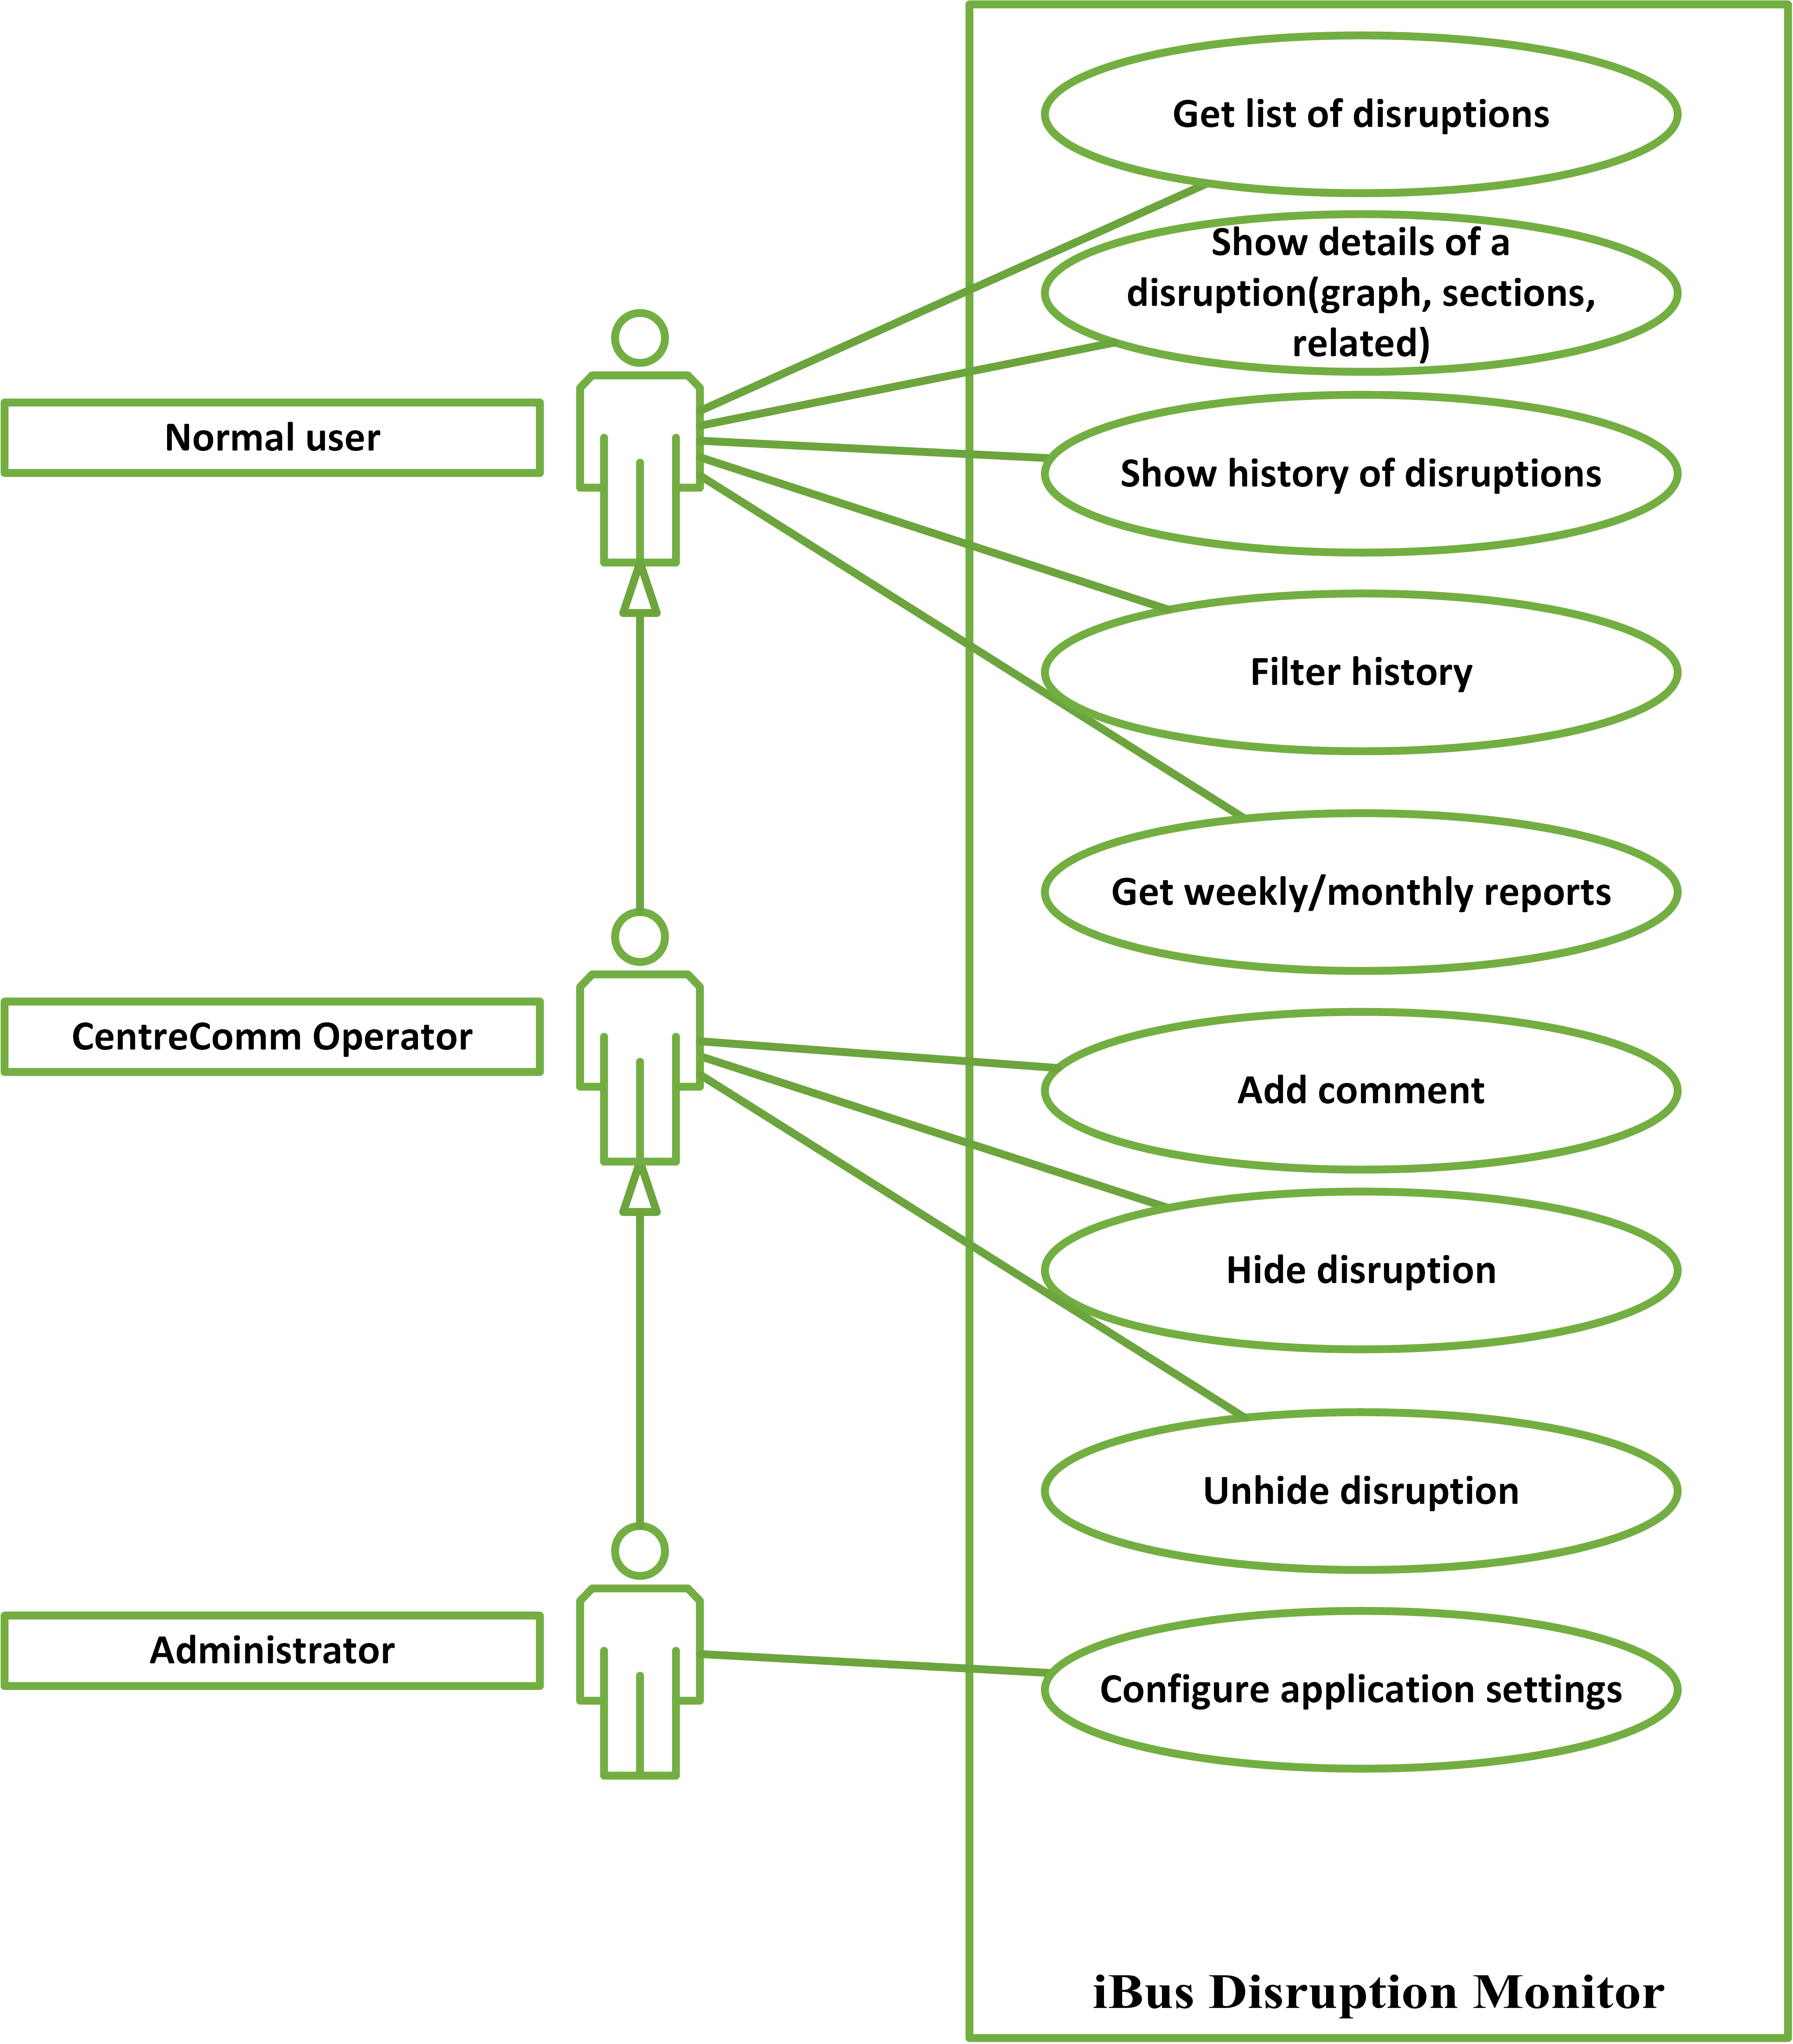
\includegraphics[width=1.2\textwidth]{Figures/UseCases.png}}
	\caption{Use Case Diagram}
\label{fig:key}
\end{figure}
%ARCHITECTURE DIAGRAM
\begin{figure}
	\makebox[\textwidth][c]{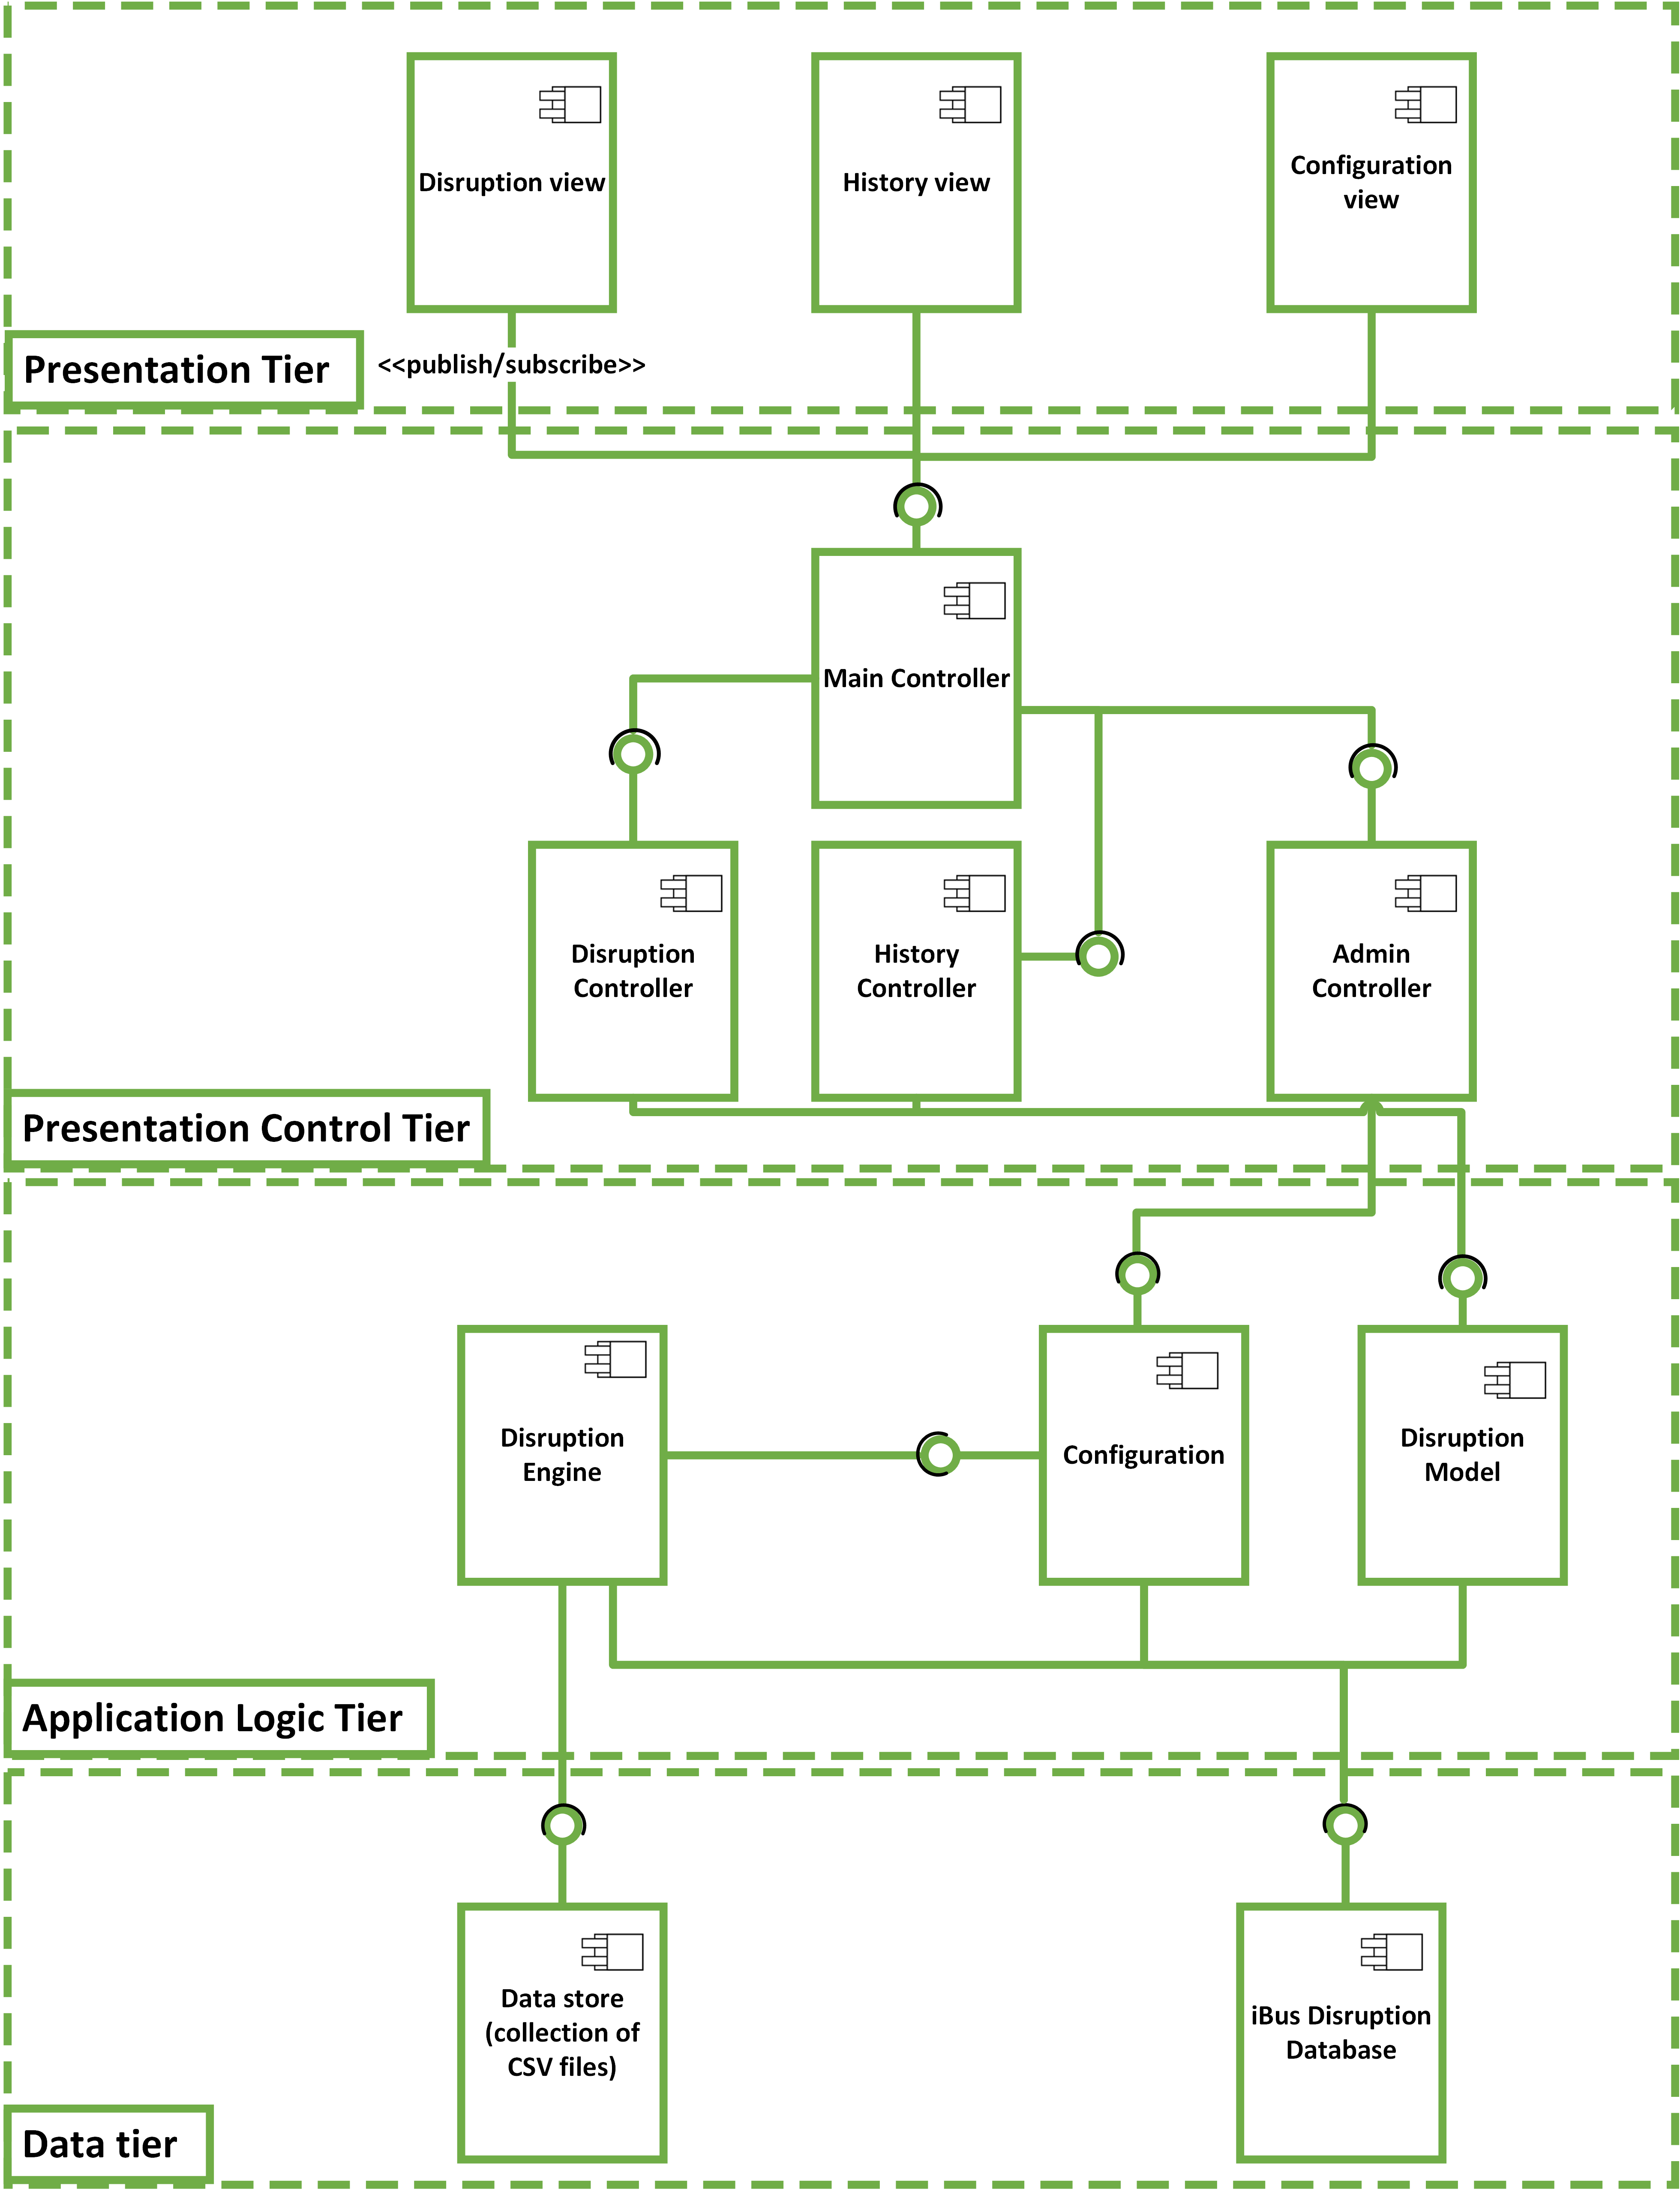
\includegraphics[width=1.2\textwidth]{Figures/Architecture.png}}
	\caption{System Architecture Diagram}
\label{fig:key}
\end{figure}
%CLASS DIAGRAM
\begin{figure}
	\makebox[\textwidth][c]{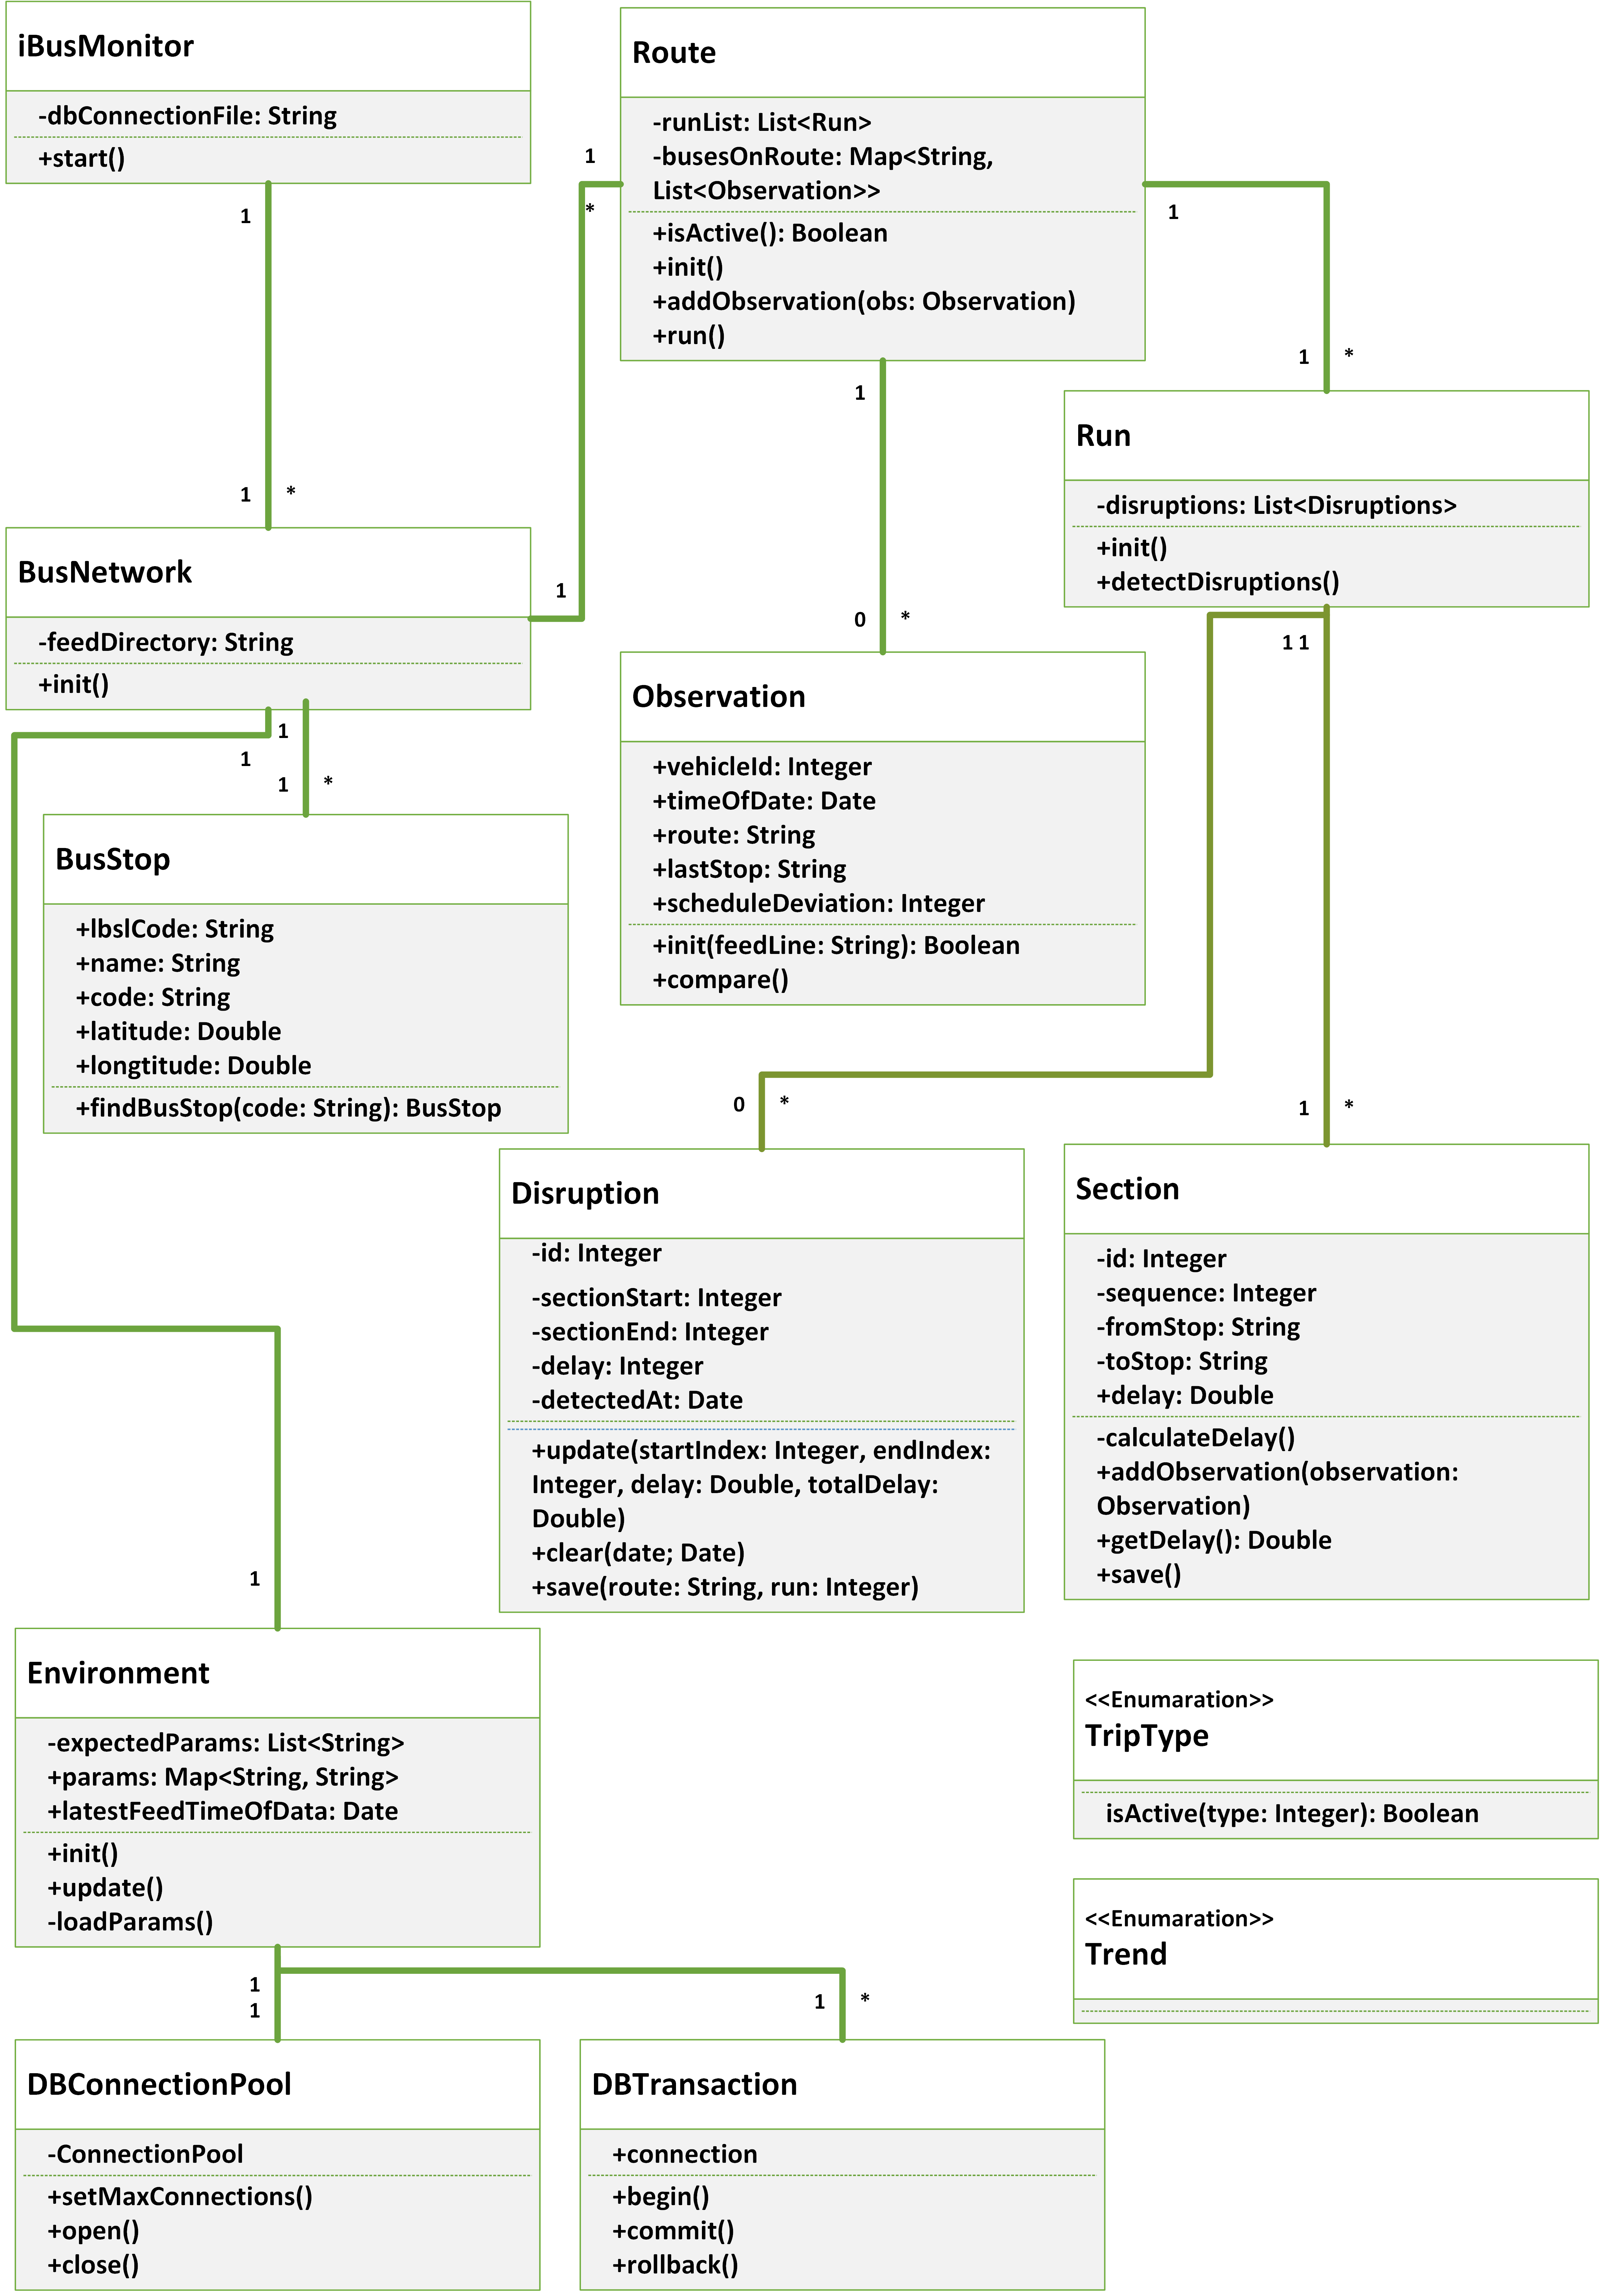
\includegraphics[width=1.2\textwidth]{Figures/Class.png}}
	\caption{Class Diagram}
\label{fig:key}
\end{figure}
%DATABSE MODEL DIAGRAM
\begin{figure}
	\makebox[\textwidth][c]{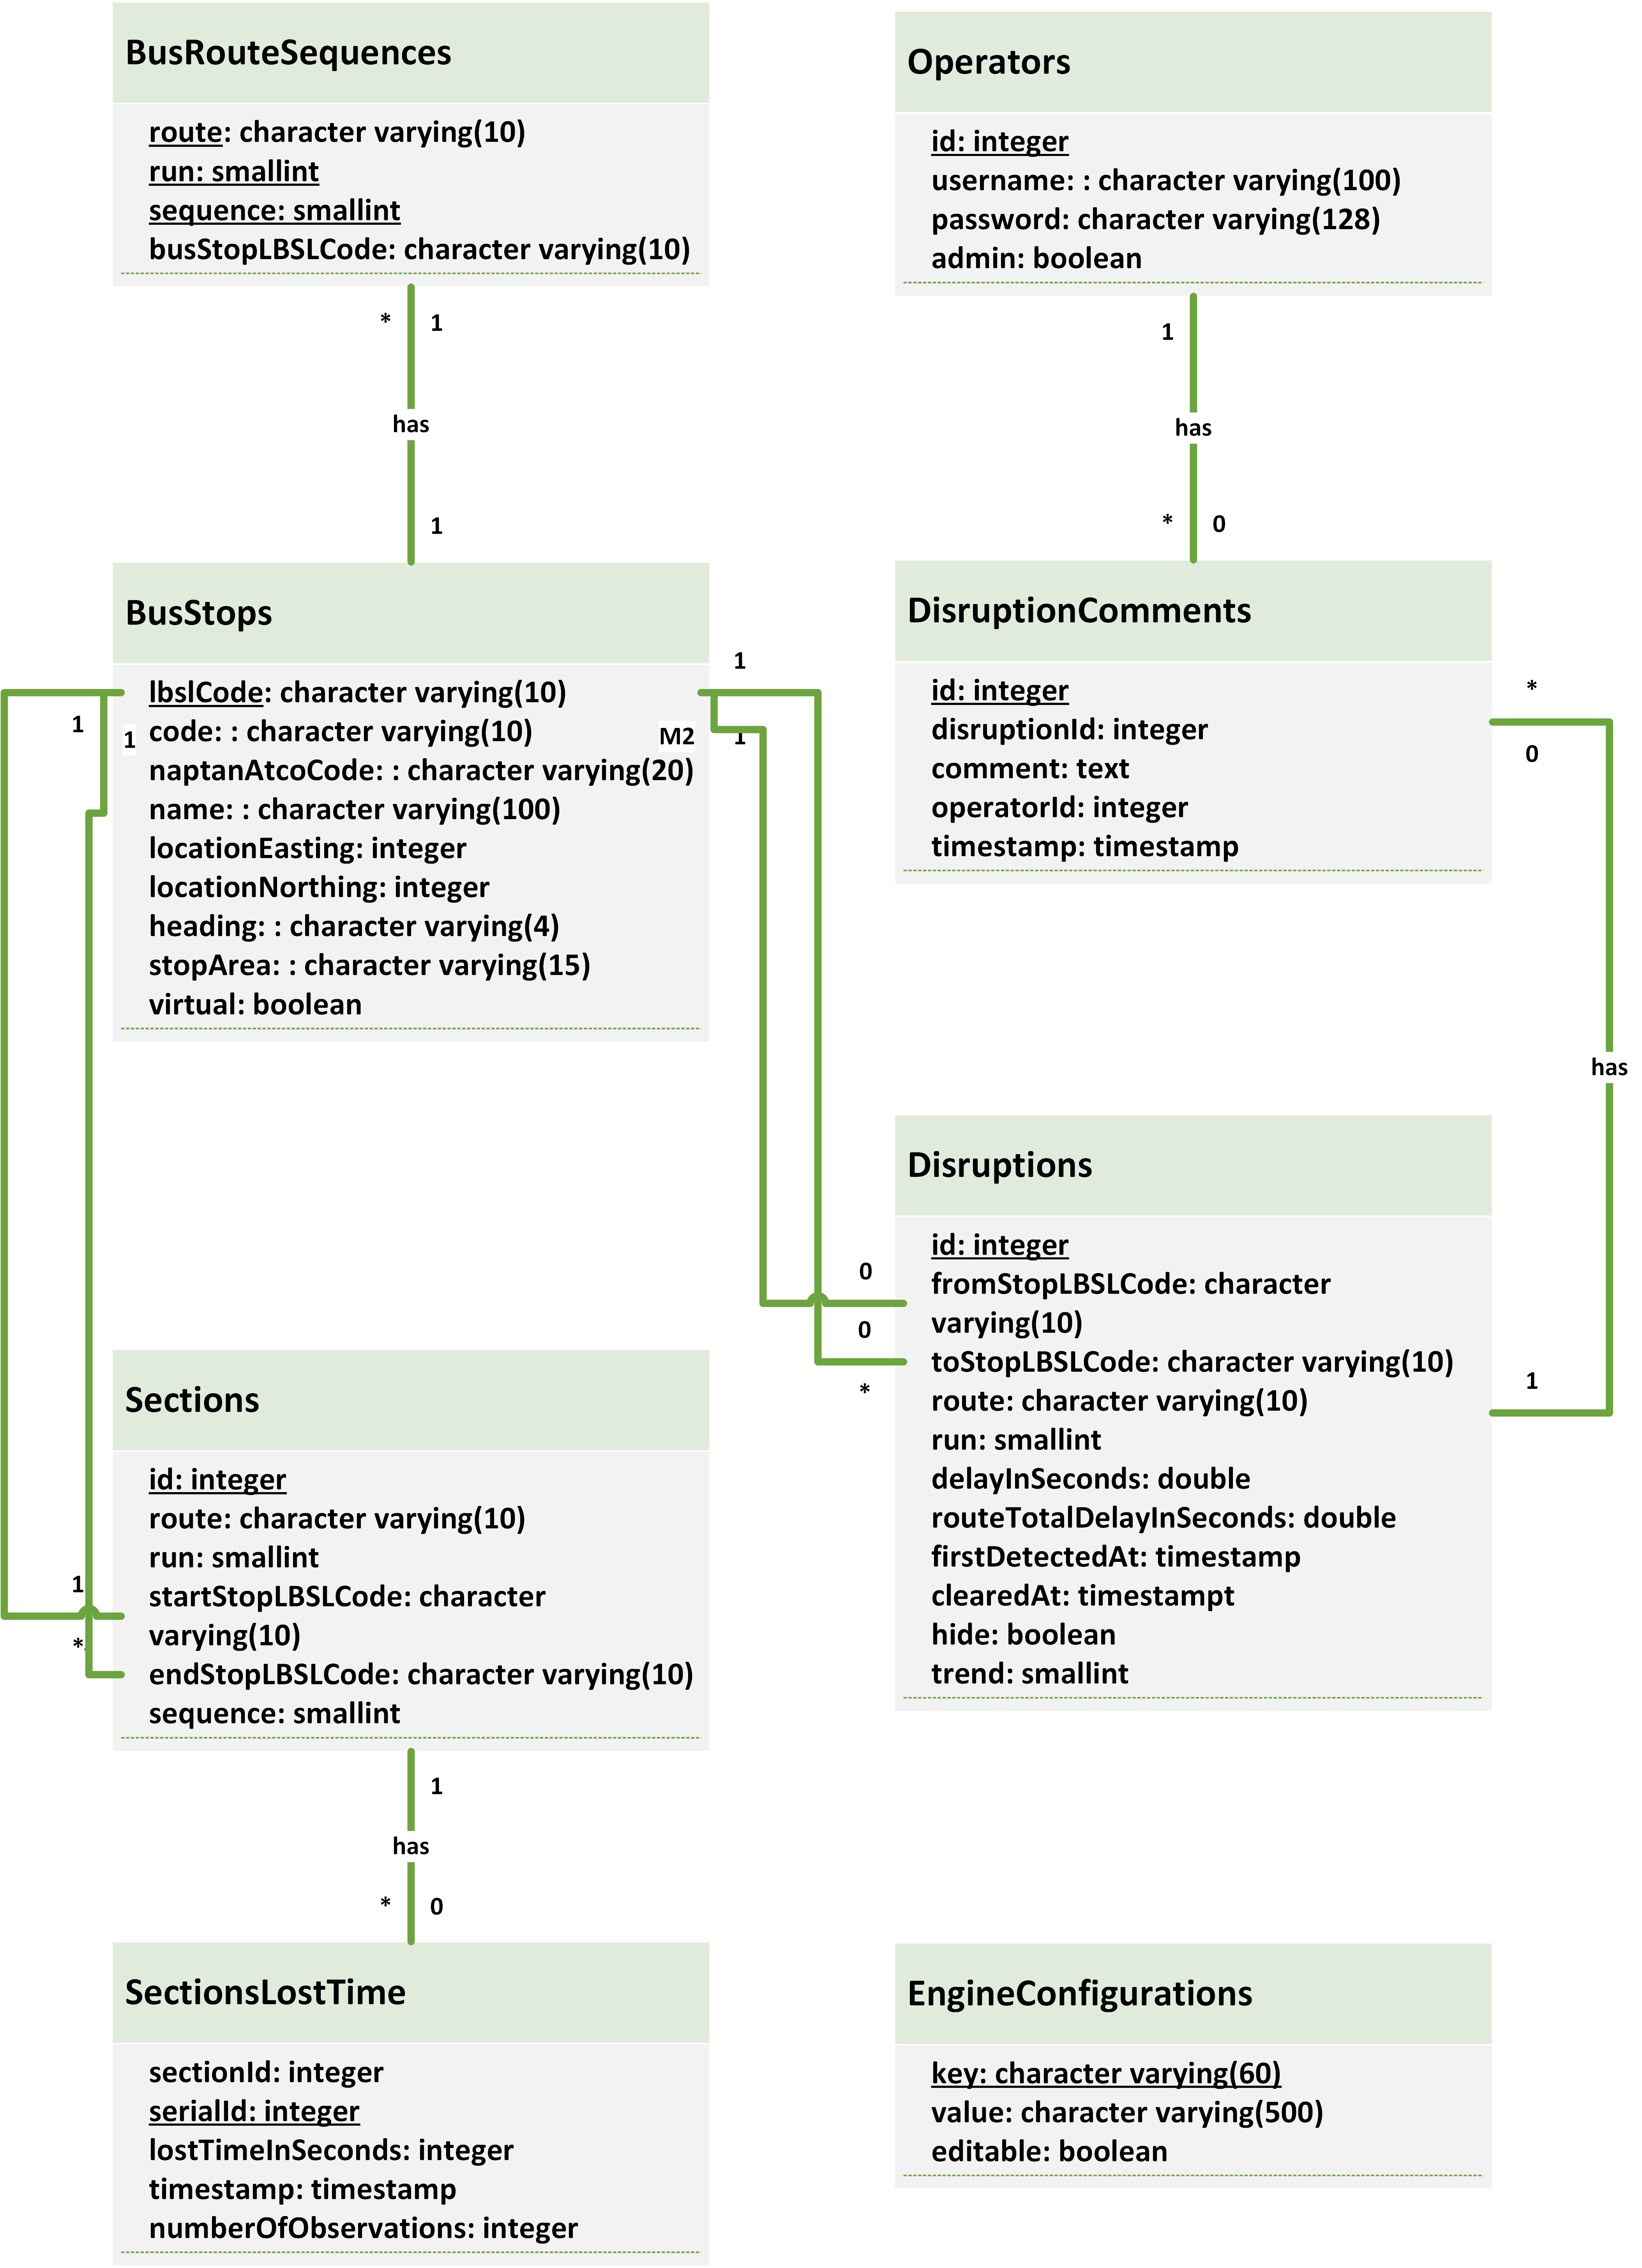
\includegraphics[width=1.2\textwidth]{Figures/DBModel.png}}
	\caption{Database Model Diagram}
\label{fig:key}
\end{figure}
%STATE MACHINE DIAGRAM
\begin{figure}
	\makebox[\textwidth][c]{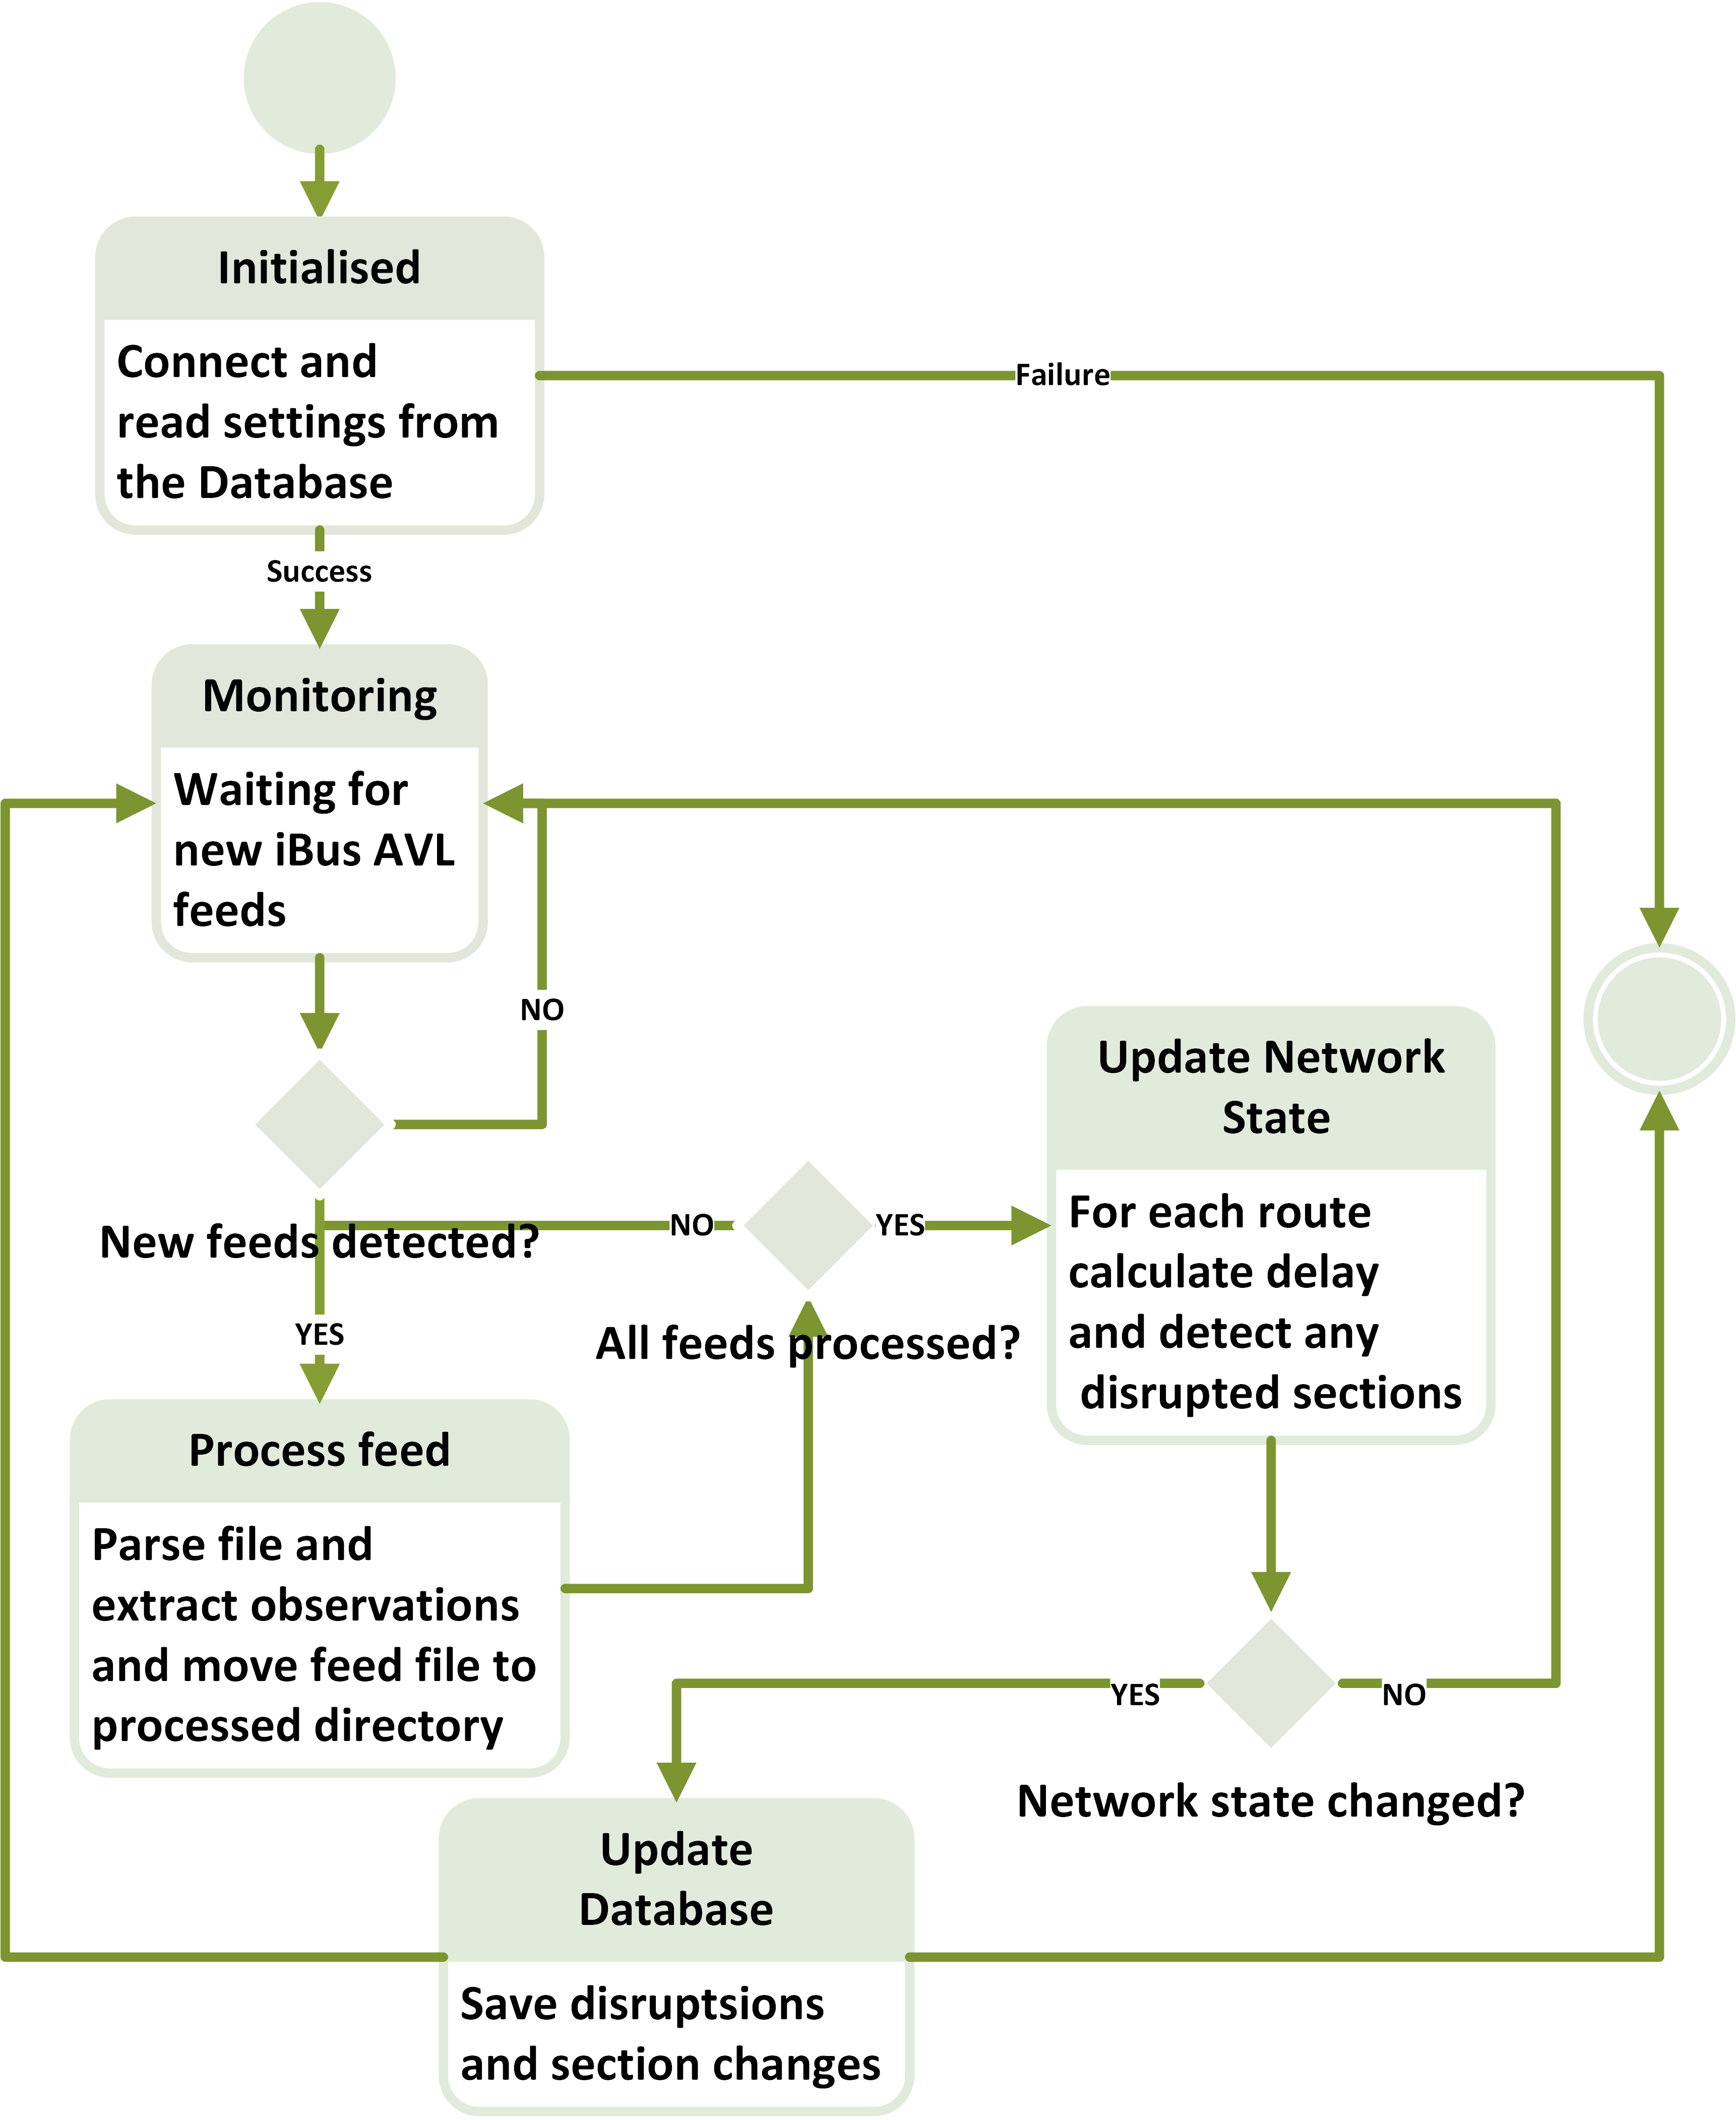
\includegraphics[width=1.2\textwidth]{Figures/StateDiagram.png}}
	\caption{State Machine Diagram}
\label{fig:key}
\end{figure}

\FloatBarrier
\section{Test Results}